% Kapitel 4 mit den entsprechenden Unterkapiteln
% Die Unterkapitel können auch in separaten Dateien stehen,
% die dann mit dem \include-Befehl eingebunden werden.
%-------------------------------------------------------------------------------
\chapter{Datenmodell}
\label{kap4}
Falls in der Anwendung bestimmte Daten dauerhaft gespeichert werden, so sind
die entsprechenden Entities und Beziehungen hier darzustellen und zu erläutern.
Dies ist insbesondere relevant, falls der Einsatz einer (relationalen)
Datenbank geplant ist.

\section{Diagramm}


\begin{figure}[H]
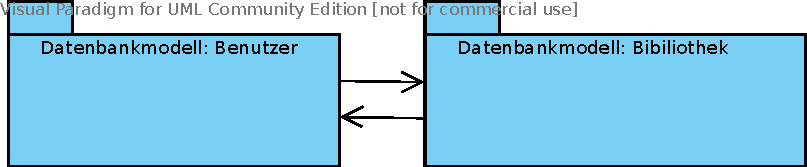
\includegraphics[width=1.0\linewidth]{bilder/db_wirelib-packages.pdf}
\caption{Datenbankmodell}
\label{fig:DBDiagramm}
\end{figure}

Das Diagramm gibt eine grobe Übersicht über die Struktur der zugrundeliegenden
relationalen Datenbank. Im Folgenden werden die beiden Teilstrukturen der
Datenbank für bessere Übersicht dargestellt.

\begin{figure}[H]
\includegraphics[width=1.0\linewidth]{bilder/database-wirelib_cluster-doc.pdf}
\caption{Datenbankmodell: Bibliothek}
\label{fig:DB_docDiagramm}
\end{figure}

Dieses Diagramm gibt eine Übersicht über alle Tabellen der Datenbank, die im
Zusammenhang mit der Bibliothek stehen. Die wichtigste Tabelle ist
\lstinline{document}, in der die vorhandenen Dokumente eingetragen werden. In
der Tabelle \lstinline{doc_status} werden alle Statusänderungen eines Dokumentes
festgehalten, einschließlich der Ausleihe eines Dokumentes. Die Tabelle
\lstinline{doc_extra} speichert zusätzliche Inhalte eines Dokumentes, die aufgrund
seltenen Gebrauchs nicht lohnen, in document direkt aufgenommen zu werden. In
der Tabelle emails werden die E-Mail-Templates gespeichert, die verschickt
werden, wenn die Ausleihfrist eines Dokumentes abläuft oder in ähnlichen
Fällen. Die Tabellen \lstinline{auth_user} und \lstinline{non_user} sind in der Teilstruktur Benutzer
und hier nur als Referenz gedacht zur besseren Übersicht. Die verbleibenden
Tabellen speichern trivialerweise den beschriebenen Inhalt.


\begin{figure}[H]

\includegraphics[width=1.0\linewidth]{bilder/database-wirelib_cluster-user.pdf}
\caption{Datenbankmodell: Benutzer}
\label{fig:DB_UserDiagramm}
\end{figure}

Dieses Diagramm gibt eine Übersicht über alle Tabellen der Datenbank, die im
Zusammenhang mit Benutzerverwaltung stehen. Alle Tabellen, die in diesem Modell
mit dem Präfix \emph{auth\_} beginnen, sind von Django generiert und werden für
eine erleichterte Handhabung von Benutzern und Rechtevergabe genutzt. Tabellen
mit dem Präfix \emph{django\_} werden ebenfalls von Django generiert und dienen
dem Admin-Interface von Django und dem Session-Managment von eingeloggten
Benutzern. Die Tabelle \lstinline{non_user} ist für Externe gedacht, die nicht
am Institut für Wissenschaftliches Rechnen arbeiten und trotzdem ein Dokument
ausleihen wollen. Sie haben so keine Möglichkeit, sich auf der Webseite
einzuloggen, können aber trotzdem Dokumente ausleihen. Die Tabellen
\lstinline{tel_user} und \lstinline{tel_non_user} werden benötigt, um
Telefonnumern zu Benutzern zu speichern.  \lstinline{user_profile} ist zur
Erweiterung der Django-Tabelle \lstinline{auth_user}, um auch Adressen
speichern zu können.

% Eigenes Klassendiagramm einsetzen
\section{Erläuterung}
Im Folgenden sind alle Relationen von einer Tabelle zu einer anderen 
in der Datenbank angezeigt. Dabei ist jeweils oben die ausgehende Tabelle und 
unter \glqq Relation zu\grqq\ alle zu denen eine Verbindung existiert. Unter 
\glqq Kardinalität\grqq\ steht dann, mit wie vielen Datensätzen der 
Relationstabelle ein Datensatz der Ausgangstabelle verbunden ist. Angegeben wird 
dabei zuerst die Mindestanzahl von Verbindungen und nach dem Komma die 
Maximalanzahl. Bei \glqq 1,n\grqq\ hat Datensatz $A$ also mindestens eine und 
maximal unendlich viele Verbindungen zur Relationstabelle.

\begin{longtable}{@{}ccc@{}}
  \toprule
  \multicolumn{3}{c}{\emph{Tabelle:} author} \\
  Relation zu & Name der Beziehung & Kardinalität \\
  \cmidrule(lr){1-1}\cmidrule(lr){2-2}\cmidrule(lr){3-3}
  document\_authors & hat geschrieben & 1,n \\
  
  \toprule
  \multicolumn{3}{c}{\emph{Tabelle:} document\_authors} \\
  Relation zu & Name der Beziehung & Kardinalität \\
  \cmidrule(lr){1-1}\cmidrule(lr){2-2}\cmidrule(lr){3-3}
  author & wurde geschrieben von & 1,1 \\
  document & hat geschrieben & 1,1\\

  \toprule
  \multicolumn{3}{c}{\emph{Tabelle:} document} \\
  Relation zu & Name der Beziehung & Kardinalität \\
  \cmidrule(lr){1-1}\cmidrule(lr){2-2}\cmidrule(lr){3-3}
  document\_authors & wurde geschrieben von & 1,n\\
  category & gehört zur Kategorie & 1,1\\
  publisher & wurde veröffentlicht von & 1,1\\
  keywords & besitzt die Schlüsselwörter & 0,n\\  
  doc\_extra & besitzt die Extrafelder & 0,n\\
  doc\_status & hat den Status/verliehen an & 0,n\\

  \toprule
  \multicolumn{3}{c}{\emph{Tabelle:} keywords} \\
  Relation zu & Name der Beziehung & Kardinalität \\
  \cmidrule(lr){1-1}\cmidrule(lr){2-2}\cmidrule(lr){3-3}
  document & gehört zum Dokument & 1,1 \\

  \toprule
  \multicolumn{3}{c}{\emph{Tabelle:} publisher} \\
  Relation zu & Name der Beziehung & Kardinalität \\
  \cmidrule(lr){1-1}\cmidrule(lr){2-2}\cmidrule(lr){3-3}
  document & hat veröffentlicht & 1,n \\

  \toprule
  \multicolumn{3}{c}{\emph{Tabelle:} category} \\
  Relation zu & Name der Beziehung & Kardinalität \\
  \cmidrule(lr){1-1}\cmidrule(lr){2-2}\cmidrule(lr){3-3}
  document & enthält & 0,n \\

  \toprule
  \multicolumn{3}{c}{\emph{Tabelle:} doc\_extra} \\
  Relation zu & Name der Beziehung & Kardinalität \\
  \cmidrule(lr){1-1}\cmidrule(lr){2-2}\cmidrule(lr){3-3}
  document & gehört zu & 1,1 \\

  \toprule
  \multicolumn{3}{c}{\emph{Tabelle:} doc\_status} \\
  Relation zu & Name der Beziehung & Kardinalität \\
  \cmidrule(lr){1-1}\cmidrule(lr){2-2}\cmidrule(lr){3-3}
  document & gehört zum Dokument & 1,1\\
  auth\_user & wurde geändert von & 1,1\\
  auth\_user & wurde ausgeliehen von & 0,1\\
  non\_user & wurde weitergegeben an & 0,1\\

  \toprule
  \multicolumn{3}{c}{\emph{Tabelle:} non\_user} \\
  Relation zu & Name der Beziehung & Kardinalität \\
  \cmidrule(lr){1-1}\cmidrule(lr){2-2}\cmidrule(lr){3-3}
  doc\_status & entlieh & 1,n\\
  tel\_non\_user & hat die Telefonnummern & 1,n\\

  \toprule
  \multicolumn{3}{c}{\emph{Tabelle:} tel\_non\_user} \\
  Relation zu & Name der Beziehung & Kardinalität \\
  \cmidrule(lr){1-1}\cmidrule(lr){2-2}\cmidrule(lr){3-3}
  non\_user & gehört zu & 1,1 \\

  \toprule
  \multicolumn{3}{c}{\emph{Tabelle:} auth\_user} \\
  Relation zu & Name der Beziehung & Kardinalität \\
  \cmidrule(lr){1-1}\cmidrule(lr){2-2}\cmidrule(lr){3-3}
  user\_profile & wohnt & 1,1\\
  tel\_user & hat die Telefonnumern & 1,n\\
  auth\_user\_user\_permissions & hat die Rechte & 0,n\\
  doc\_status & änderte den Status & 0,n\\  
  doc\_status & leiht/bürgt gerade für & 0,n\\
  django\_admin\_log & aktualisiert & 0,n\\
  auth\_message & bekam & 0,n\\
  auth\_user\_groups & ist in Gruppe & 0,n\\

  \toprule
  \multicolumn{3}{c}{\emph{Tabelle:} tel\_user} \\
  Relation zu & Name der Beziehung & Kardinalität \\
  \cmidrule(lr){1-1}\cmidrule(lr){2-2}\cmidrule(lr){3-3}
  auth\_user & gehört zu & 1,1 \\

  \toprule
  \multicolumn{3}{c}{\emph{Tabelle:} auth\_message} \\
  Relation zu & Name der Beziehung & Kardinalität \\
  \cmidrule(lr){1-1}\cmidrule(lr){2-2}\cmidrule(lr){3-3}
  auth\_user & gesendet an & 1,1 \\

  \toprule
  \multicolumn{3}{c}{\emph{Tabelle:} user\_profile} \\
  Relation zu & Name der Beziehung & Kardinalität \\
  \cmidrule(lr){1-1}\cmidrule(lr){2-2}\cmidrule(lr){3-3}
  auth\_user & Anschrift von & 1,1 \\

  \toprule
  \multicolumn{3}{c}{\emph{Tabelle:} auth\_user\_groups} \\
  Relation zu & Name der Beziehung & Kardinalität \\
  \cmidrule(lr){1-1}\cmidrule(lr){2-2}\cmidrule(lr){3-3}
  auth\_user & der User & 1,1 \\
  auth\_group & gehört zur Gruppe & 1,1 \\

  \toprule
  \multicolumn{3}{c}{\emph{Tabelle:} auth\_group} \\
  Relation zu & Name der Beziehung & Kardinalität \\
  \cmidrule(lr){1-1}\cmidrule(lr){2-2}\cmidrule(lr){3-3}
  auth\_user\_groups & besitzt die Mitglieder & 0,n \\
  auth\_group\_permissions & hat die Rechte & 0,n \\

  \toprule
  \multicolumn{3}{c}{\emph{Tabelle:} auth\_group\_permissions} \\
  Relation zu & Name der Beziehung & Kardinalität \\
  \cmidrule(lr){1-1}\cmidrule(lr){2-2}\cmidrule(lr){3-3}
  auth\_group & die Gruppe & 1,1 \\
  auth\_permission & hat das Recht & 1,1 \\

  \toprule
  \multicolumn{3}{c}{\emph{Tabelle:} auth\_user\_user\_permissions} \\
  Relation zu & Name der Beziehung & Kardinalität \\
  \cmidrule(lr){1-1}\cmidrule(lr){2-2}\cmidrule(lr){3-3}
  auth\_user & der User & 1,1 \\
  auth\_permission & hat das Recht & 1,1 \\

  \toprule
  \multicolumn{3}{c}{\emph{Tabelle:} auth\_permission} \\
  Relation zu & Name der Beziehung & Kardinalität \\
  \cmidrule(lr){1-1}\cmidrule(lr){2-2}\cmidrule(lr){3-3}
  auth\_user\_user\_permissions & der User hat  & 0,n \\
  auth\_group\_permissions & die Gruppe hat & 0,n \\
  django\_content\_type & referenziert & 1,1 \\

  \toprule
  \multicolumn{3}{c}{\emph{Tabelle:} django\_admin\_log} \\
  Relation zu & Name der Beziehung & Kardinalität \\
  \cmidrule(lr){1-1}\cmidrule(lr){2-2}\cmidrule(lr){3-3}
  auth\_user & getätigt von  & 1,1 \\
  django\_content\_type & referenziert & 1,1 \\

  \toprule
  \multicolumn{3}{c}{\emph{Tabelle:} django\_content\_type} \\
  Relation zu & Name der Beziehung & Kardinalität \\
  \cmidrule(lr){1-1}\cmidrule(lr){2-2}\cmidrule(lr){3-3}
  auth\_permission & stellt Referenz  & 0,n \\
  django\_admin\_log & ändert & 0,n \\
\end{longtable}
